\chapter{Development}
The goal of this chapter is to illustrate the new implementations and changes to the project's software, describing the improvements of the previous features, the new ones and the way in which they have been achieved.
\bigbreak

In the previous project's code, some time and memory optimizations have been made, minor bugs have been found and fixed and some other improvements have been done (e.g. replacing deprecated methods and libraries with newer ones).

\section{MQTT QoS2 caching}
As mentioned in the \textit{Unsolved Issues} chapter of Dario Piotrowicz's thesis \cite{Pio19}, there was a problem with unreliable Wi-Fi networks (an issue in the library's GitHub repository is still open \cite{githubQos2Issue}): all messages generated while a broken client-broker connection were discarded, instead of being stored to be sent when the connection will be re-established.

To solve that issue have been implemented two caching queues, one for each connection: the playing session one and the neural network's pattern collection one.

The cache size has been set to a safe value of 32 kilobytes (tested experimentally: bigger values led the Photon out of memory more often than not). The maximum number of messages that can be cached is stored in the \texttt{cache\_size} variable. With a maximum message size of 512 characters (511 effective characters because of the null terminator), the value is easily calculated as 32.

The following is a graph of the playing session's connection caching implementation; the neural network one is analogous.
\bigbreak

\begin{lstlisting}[style=CPPStyle]

	...

	// ready to send the data (publishString) to the client
	if (client.isConnected()) {
        while (cached_messages.size() > 0) {
			// send cached messages
            std::string msg = cached_messages.front();
            cached_messages.pop();
			client.publish("motiontracker/" + ID,
							msg.c_str(),
							MQTT::QOS2);
        }
		client.publish("motiontracker/" + ID,
						publishString,
						MQTT::QOS2);
    } else if (cached_messages.size() < cache_bound) {
		// save message in cache
        std::string msg(publishString);
        cached_messages.push(msg);
    }

	...

\end{lstlisting}
\bigbreak

This solution has made possible to damper temporary disconnections caused by instable connections.

\section{Delay in real-time data plotting}
\dots

\section{Motion capture}
In the software's previous version, developed and improved by Dario Piotrowicz \cite{Pio19} from the Marco Lanini's project \cite{Lan17}, the data processed by the device and sent to the server were:
\begin{itemize}
	\item device's orientation both in quaternions and yaw, pitch and roll angles;
	\item device's acceleration in Cartesian and spherical coordinates system;
	\item raw accelerometer, gyroscope and magnetometer data;
	\item device's velocity approximation.
\end{itemize}

This work's aim is to detect \textit{discriminating features among different playing patterns}, by collecting and analyzing the sensors data stream; the analysis followed the flow in the data fusion schema (Figure \ref{old data fusion schema}), except for the velocity approximation.
\bigbreak

The velocity approximation, calculated by the \textit{Velocimeter} class \cite{Pio19}, was early excluded because of the practical difficulty in obtaining realistic values using only inertial sensors, where measurement errors are unavoidable, especially for miniature MEMS sensors \cite{Du15, Est14, Kow15, Liu01, Sei07, UsingAcc, Woo07, Yan06}.

Direct integration of acceleration often causes unrealistic drifts in velocity, due to errors propagation; furthermore, measured acceleration not only carries random noise, but also presents with offset caused by temperature drift \cite{Kow15, Liu01, Woo07}, resulting in estimation errors accumulated by integration process, that results in low accuracy.

In particular, two behaviors were miscalculated:
\begin{itemize}
	\item stillness after a movement: if the truck toy is pushed from behind and it is left to stop alone, the velocity is expected to linearly decrease down to zero, but the velocity graph shows an uniform-like decrease in the first phase, and a peak towards zero in the last one;
	\item repetitive light accelerations: the vertical acceleration generated by the tessellated tyres rolling resulted in absent vertical velocities.
\end{itemize}

\begin{center}
	\begin{figure}[ht]
		\makebox[\textwidth]{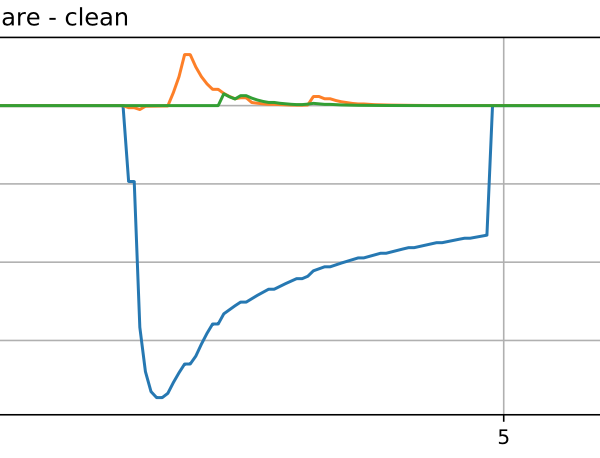
\includegraphics[width=0.2\paperwidth]{img/plots/square.png}}
		\caption{Square wave and absent velocities.}
	\end{figure}
\end{center}

\subsection{Gravity-affected data}
The first analytic phase dealt with raw accelerometer data, but the signal's noisiness and the presence of gravity have induced to desist. Nevertheless, especially for movements with strong accelerations, that simply increase the signal-to-noise ratio, the main waveform was recognizable.
\bigbreak

TODO: graph
\bigbreak

The analysis moved to Kalman-filtered data, which proved to be much cleaner and smoother, but still influenced by gravity; thus it would have been necessary a more complex training data collection, due to the lack of orientation invariance – the gravity decomposes among the axes in accordance with device's orientation, influences other accelerations, and affects the neural network's training: the neural network would believe that the gravity is part of the pattern acceleration; consequently, the same pattern recorded with a different device's orientation would be classified differently. To achieve such invariance it would be necessary to collect every pattern with the device rotated in any possible angle.
\bigbreak

TODO: graph
\bigbreak

Nevertheless, it was discovered that the gravity-free acceleration computed by the device and sent to the server was not stored in the database, but only used for the 3D visual representation. It was decided to store such data in the database along with other sensors data, and analyze it to see whether it was reliable over time. A smooth gravity-free acceleration could have been the turning point for an efficient neural network training and future classification.
\bigbreak

\subsection{Gravity-free data}
Analyzing gravity-free data, another problem showed up: after a few minutes of playing, the calculation of the yaw angle accumulated errors that led it to diverge in an unrealistic way, rotating counterclockwise, and consequently the accelerations no longer matched the device's orientation. The error didn't grow with the still device, but only when the device was moved, and therefore it should not be confused with the \textit{yaw drift} problem, that leads the yaw to rotate constantly in any device condition, and it's often caused by biases in gyroscope measurements (and that's the case of this project \cite{Pio19}) or poor/absent magnetometer calibration.
\bigbreak

The yaw's measurement was particularly affected by rotations around the Earth's $z$-axis (in other words, over the plane generated by the $x$ and $y$ axes), and the bigger the pitch angle, the bigger the error, as shown in the table below. Pitch and roll, on the contrary, were calculated almost without errors.
\bigbreak

\begin{table}[ht!]
	\centering
	\begin{tabular}{c|c c}
	\textbf{Pitch} ($^{\circ}$) & \textbf{Mean error} ($^{\circ}$) & \textbf{Standard deviation} ($^{\circ}$) \\ \hline
	0                           & -47.12                           & 0.94                                     \\
	20                          & -47.67                           & 1.88                                     \\
	40                          & -51.14                           & 1.45                                     \\
	60                          & -58.14                           & 1.73                                     \\
	80                          & -57.80                           & 0.75
	\end{tabular}
	\caption{Yaw errors after a 360$^{\circ}$ rotation with different pitch angles.}
\end{table}

Small yaw variations were also noticed with pitch-only movements: after a 360$^{\circ}$ rotation, the mean error was 0.47$^{\circ}$ with a standard deviation of 0.11$^{\circ}$.

\begin{center}
	\begin{figure}[ht]
		\makebox[\textwidth]{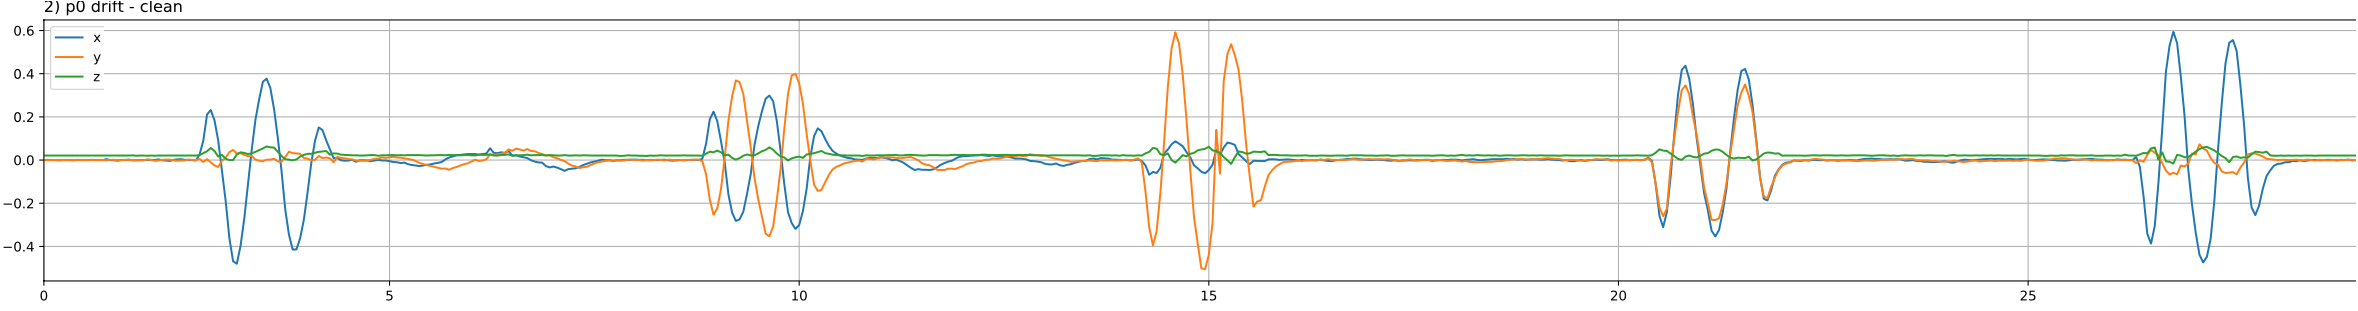
\includegraphics[width=0.7\paperwidth]{img/plots/drift.png}}
		\caption{Different accelerations for the same pattern.}
	\end{figure}
\end{center}

During some tests, it was noticed another unexpected behavior: different recordings of the same pattern with different device rotations showed the same acceleration among axes (e.g. given a fixed three-dimensional path, following it with the truck facing forwards, backward, upside-down or other, would show exactly the same accelerations).
\bigbreak

TODO: Plot with the same movement with different orientations that shows the same data
\bigbreak

The cause of the error was discovered to be in the Madgwick's algorithm implementation, more precisely in the lack of yaw's convergence in its error-correction gradient descent phase (see section \ref{Madgwick filter}). Unfortunately, several algorithm implementations that included the correction, and different values of the algorithm's gain parameter (the magnitude $\beta$ of the gyroscope measurement error\footnote{Increasing $\beta$ leads to faster bias corrections and higher sensitiveness to lateral accelerations.} \cite[13]{Mad10}) gave no better results over time, and worse, ghost accelerations were found. Then, the Lanini's version has been kept and the troubleshooting continued.
\bigbreak

Since the accelerations were independent from the orientation of the device, the cause was necessarily the reference system's location, which proved to be global: the movements were shown as viewed by an external observer, placed in the Earth's center.

To align the reference system back, it was sufficient to rotate the acceleration vector by the 3 orientation angles (of \textit{yaw}, \textit{pitch} and \textit{roll}) given by the Madgwick's algorithm, and that, as shown below, not only correctly brought the reference system back to a local point of view, but surprisingly solved the yaw alignment issue.

The explanation of this (apparent) side-effect lies in how the gravity subtraction is performed: as shown in the Figure \ref{old data fusion schema}, the data obtained from the Kalman and Madgwick filters are used jointly. As discussed above, the Kalman filter does not present any problem, while the Madgwick one fails in the yaw angle calculation; hence, the resulting acceleration is misaligned, and needs to be corrected by the same misalignment angle: the Madgwick's angle itself.
\bigbreak

The rotation of the acceleration vector has been performed through a three-dimensional rotation matrix. In three-dimensional matrices, the matrix-vector multiplication doesn't affect the speed meaningfully, even for relatively weak CPUs like the one that runs in the Photon: the goal packets' frequency of 22 Hertz \cite{Pio19} has been always achieved (when the wireless connection allowed it) and however the C++ code is compiled by \texttt{GCC} with the \texttt{-Os} flag, that includes the loop unrolling optimization \cite{UsingGCC}.

\begin{center}
	\begin{figure}[ht]
		\makebox[\textwidth]{
\includegraphics[width=0.7\paperwidth]{img/plots/nodrift.png}}
		\caption{Image of correct accelerations.}
	\end{figure}
\end{center}

\subsection{Fine tuning: magnetic distortions}
Once achieved a reliable gravity-filtered acceleration approximation, it was possible to perform some fine tuning.
\bigbreak

It is known that magnetic and inertial sensors can be influenced by magnetic disturbance \cite{Fan17}.
There are two types of magnetic distortions:
\begin{enumerate}
	\item \textit{soft iron}: it's a temporary influence that appears when a material is affected by the Earth's magnetic field, and it's induced from metals that are non permanently magnetised (they don't generate a magnetic field themselves) \cite{Cro15}. It causes errors in the measured direction of the Earth's magnetic field, and since it depends on the orientation of the material relative to the sensor and the magnetic field, it cannot be compensated by a constant \cite{CompensatingIron};
	\item \textit{hard iron}: it's produced by materials that exhibit a constant, additive field to the Earth's magnetic field \cite{CompensatingIron}, and it can be simply removed by a constant offset, calculated through calibration \cite{CompensatingIron, Geb06, Kok12}.
\end{enumerate}

Madgwick's algorithm is able to remove \textit{soft iron} distortions \cite[11-12]{Mad10}, and the calibration to remove \textit{hard iron} distortions has been performed by the SparkFun's Arduino library.
\bigbreak

Unfortunately, there are non-constant interferences that still affect the sensors readings, such as the magnetic field generated by the current passing through the USB cable for charging the battery.
Its removal is much harder, because requires to analyze how much current is flowing through the cable, and the knowledge of the net magnetic field's shape, that depends on how the cable is placed around the sensor.

\begin{center}
	\begin{figure}[ht]
		\makebox[\textwidth]{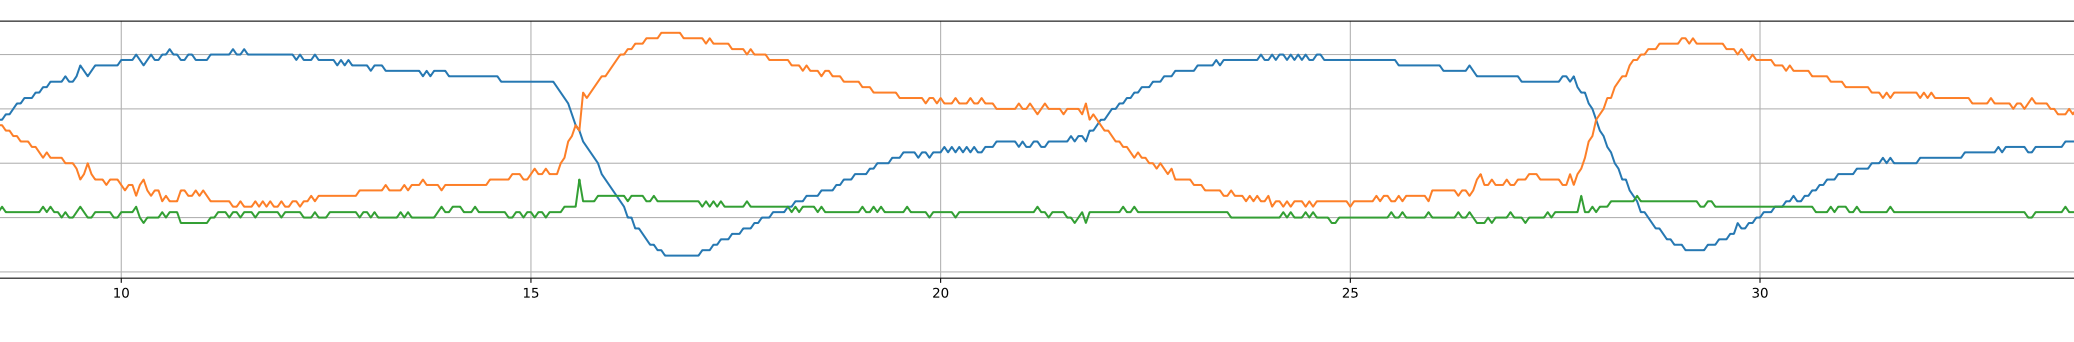
\includegraphics[width=0.7\paperwidth]{img/plots/battery.png}}
		\caption{Orientation affected by the battery charging.}
	\end{figure}
\end{center}

\subsection{Final data schema}
The current data flow is illustrated by the schema:

\begin{center}
	\begin{figure}[ht]
		\makebox[\textwidth]{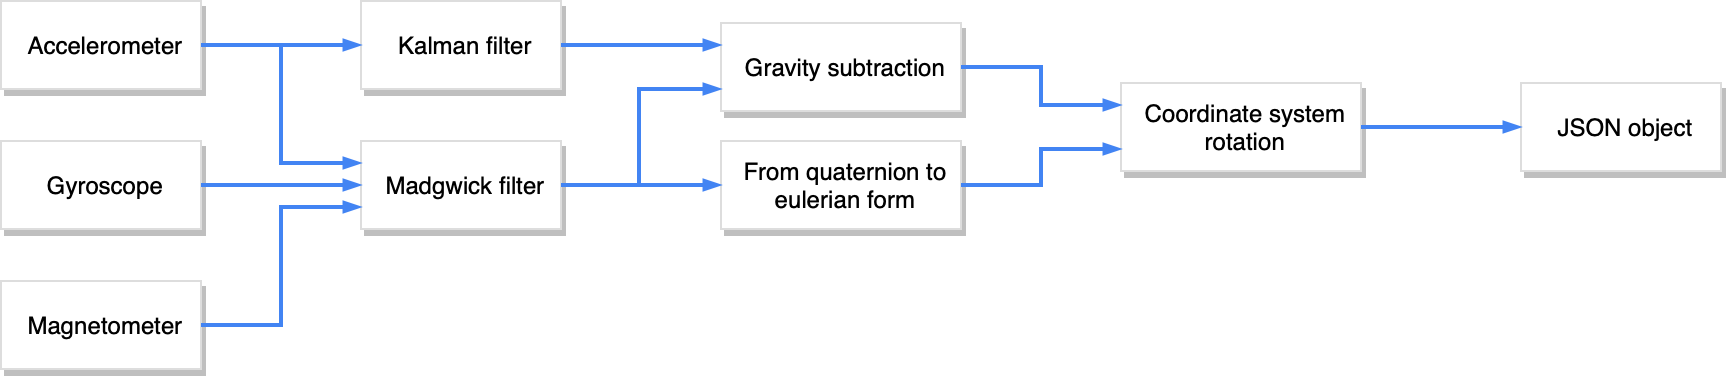
\includegraphics[width=0.65\paperwidth]{img/data_fusion.png}}
		\caption{Current data fusion schema.}
	\end{figure}
\end{center}

\section{Pattern recognition}
Pattern recognition can be formally defines as \textit{the process whereby a received pattern/signal is assigned to one of a prescribed number of classes} \cite{Hay08}.

In general, pattern recognition using neural networks may take one of two forms \cite{Hay08}:
\begin{itemize}
	\item there is one unsupervised 
\end{itemize}
